\documentclass{article}
\usepackage{graphicx}
\usepackage{hyperref}
\usepackage{changepage}
\usepackage{tikz}
\usepackage{tgtermes}
\usepackage{amsfonts}

\usepackage{fancyhdr}
\pagestyle{fancy}

\renewcommand{\headrulewidth}{0pt}

% Cabeçalho
\fancyhead[L]{DCC 207} % topo esquerdo
\fancyhead[R]{Geometrial Computacional} % topo direito

% Rodapé
\fancyfoot[L]{Trabalho Prático I} % rodapé esquerdo
\fancyfoot[R]{Outono 2025} % rodapé direito

% (Opcional) limpa o centro
\fancyhead[C]{}
\fancyfoot[C]{\thepage} % página no centro do rodapé

\begin{document}

\begin{center}
    {
    \Large
    Trabalho Prático I - Geometria Computacional

    DCC 207 - Algoritmos II
    
    }

    Departamento de Ciência da Computação, Instituto de Ciências Exatas, Universidade Federal de Minas Gerais

    Belo Horizonte, Minas Gerais

    Outono de 2025
\end{center}

\begin{flushright}
2022101086  Augusto Guerra de Lima\\
\href{mailto:augustoguerra@dcc.ufmg.br}{\texttt{augustoguerra@dcc.ufmg.br}}\\
2023028234  Cauã Magalhães Pereira\\
\href{mailto:caua.magalhaes@dcc.ufmg.br}{\texttt{caua.magalhaes@dcc.ufmg.br}} \\
2023028579  Heitor Gonçalves Leite\\
\href{mailto:heitorleite@dcc.ufmg.br }{\texttt{heitorleite@dcc.ufmg.br }}
\end{flushright}
\vspace{1cm}

\begin{adjustwidth}{-1.5cm}{-1.5cm}

\section{Introdução}
\ 

Este trabalho objetiva estudar como estruturas de dados associadas a geometria computacional, a saber, árvores \(k\)-dimensionais, são empregadas no contexto de georreferenciamento.

\section{Metodologia}
\subsection{Coleta e processamento de dados}

\subsection{Estrutura de dados, árvore k-dimensional}
\ 

Árvores \(k\)-dimensionais dividem o conjunto \(P\) de pontos em partições. Seja \(p \in P\) um ponto tal que \(p=(x_1,x_2,...,x_k)\), isto é, possui \(k\) coordenadas, a estrutura de dados particiona recursivamente o espaço alternando entre suas dimensões, de forma a comparar apenas uma dimensão específica por nível, resultado em uma \textit{árvore binária}.

Em particular, nos dados geográficos, as coordenadas \textit{latitude} e \textit{longitude} implicam em uma árvore bidimensional (\(2d\)\textit{-tree}); De forma que, se no nível \(l\) é utilizada a coordenada \(x_1\) para o particionamento, em \(l+1\) tão somente, será utilizada a coordenada \(x_2\), tal que \((x_1,x_2) \in \texttt{float}^2\).

A propósito, seja \(a=(a_1,a_2),\ b=(b_1,b_2) \in \texttt{float}^2\), duas coordenadas tal que \(a_1\leq b_1\) e \(a_2 \leq b_2\), o conceito de \textit{busca intervalar ortogonal} surge naturalmente: Constitui-se em determinar um subconjunto de pontos \(P'=\{p_1,p_2,...,p_n\} \subset \texttt{float}^2\), onde 
para todo \(p \in P'\), \(a \leq p \leq b\); Com a adição de que busca é definida em retângulos paralelos aos eixos.

Como mostrado em \cite{md}, a \textit{busca intervalar ortogonal} tem uma propriedade útil, designadamente pode ser decomposta em produto de \textit{buscas intervalares unidimensionais}. Justificando a rotatividade de coordenadas.
\[\{p \in \texttt{float}^k : a_i \leq p_i \leq b_i\} = [a_1,b_1] \times[a_2,b_2] \times ... \times [a_k, b_k].\]

\begin{figure}[h]
\centering
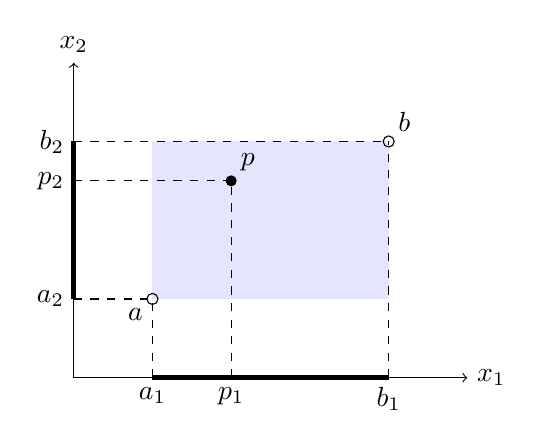
\begin{tikzpicture}
  \draw[->] (0,0) -- (5,0) node[right] {$x_1$};
  \draw[->] (0,0) -- (0,4) node[above] {$x_2$};

  \fill[blue!10] (1,1) rectangle (4,3);
  \draw[line width=2pt] (0,1)--(0,3);
  \draw[line width=2pt] (1,0)--(4,0);
  \draw[dashed] (1,0) -- (1,1);
  \draw[dashed] (4,0) -- (4,3);
  \draw[dashed] (0,1) -- (1,1);
  \draw[dashed] (0,3) -- (4,3);

  % Labels
  \node at (1,0) [below] {$a_1$};
  \node at (4,0) [below] {$b_1$};
  \node at (0,1) [left] {$a_2$};
  \node at (0,3) [left] {$b_2$};
  \node at (1,1) [below left] {$a$};
  \node at (4,3) [above right] {$b$};

  % Point p
  \draw (1,1) circle (2pt);
  \draw (4,3) circle (2pt);
  \fill (2,2.5) circle (2pt);
  \draw[dashed] (2,0) -- (2,2.5);
  \draw[dashed] (0,2.5) -- (2,2.5);
  \node at (2,2.5) [above right] {$p$};
  \node at (2,0) [below] {$p_1$};
  \node at (0,2.5) [left] {$p_2$};
\end{tikzpicture}
\caption{Representação de uma busca intervalar ortogonal em um espaço bidimensional arbitrário.}
\end{figure}




\subsubsection{Análise de complexidade}

\section{Resultados}

\section{Considerações finais}

\section{Bibliografia}

\begin{thebibliography}{99}

\bibitem[GB]{guibas}
Leonidas J. Guibas. \textit{Geometric Range Searching
Kinetic Data Structures
Clustering Mobile Nodes}; Stanford University. Disponível em: \url{https://graphics.stanford.edu/courses/cs428-03-spring/03Talks/Range.pdf}. Acesso em: 1 jun. 2025.

\bibitem[MD]{md}
MOUNT, Dave. CMSC 754: \textit{Lecture} 14 \textit{- Orthogonal Range Searching and kd-Trees}; University of Maryland. Disponível em: \url{https://www.cs.umd.edu/class/fall2021/cmsc754/Lects/lect14-kd-tree.pdf}. Acesso em: 1 jun. 2025.

\end{thebibliography}




\end{adjustwidth}
\end{document}